\subsubsection{Image Analysis Techniques}
	There are multiple techniques which can be applied to imagery to extract information which include detection of edges or objects and using known data to take measurements. These methods tend to compare data from neighbouring pixels to spot differences which can indicate features.
	\paragraph{Edge Detection}
	This is the application of mathematical algorithms to locate and highlight the edges of features in an image. There are multiple algorithms which can be used for edge detection including Sobel, Roberts, Canny, and fuzzy logic though all utilise the concept of comparing side by side pixel data to find "steps" from one brightness to another.
	\begin{table}[h!]
		\centering
		\caption{Table of pixel data showing an edge}
		\label{tab:edgePixels}
		\begin{tabular}{|c|c|c|c|c|c|c|}
			\hline
			5&7&6&4&152&148&149\\
			\hline
			\cellcolor[HTML]{0D0D0D}&
			\cellcolor[HTML]{121212}&
			\cellcolor[HTML]{0F0F0F}&
			\cellcolor[HTML]{0a0a0a}&
			\cellcolor[HTML]{989898}&
			\cellcolor[HTML]{949494}&
			\cellcolor[HTML]{959595}\\
			\hline
		\end{tabular}
	\end{table}\\
	Table \ref{tab:edgePixels} represents possible pixel values of an edge indicated by the large difference between 4 and 152. The applied algorithm will pick up on this discrepancy and in will be indicated on the resulting image. A common application for edge detection is text recognition such as in automatic number plate recognition (ANPR) \citep{anpr} as the process can remove unwanted background data and highlight the block shapes of the number plate. Figure \ref{fig:anpr} shows an image which has had thresholding applied with the number plate of the car clearly visible.
	\begin{figure}[h!]
		\centering
		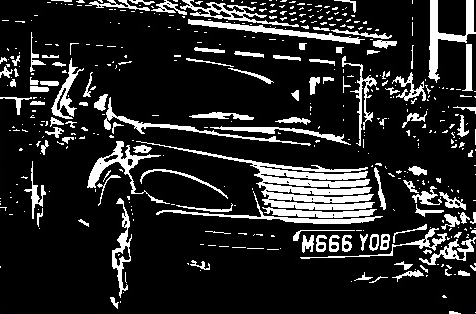
\includegraphics[width=10cm]{../images/anpr.jpg}
		\caption{Edge detection applied to an image for number plate recognition}
		\label{fig:anpr}
	\end{figure} 
	\paragraph{Hough Transform}\todo{complete hough transform section}
	Originally created in 1962 by Paul Hough, the Hough transform methods offer techniques for the discovery of features within images which includes features with imperfections. The original algorithms were created for the detection of lines but have since been improved and adapted to find circles, ellipses, and other basic shapes.
	\\\\
	Edge detection is suitable to highlight points in an image clearly though issues with the base image such as incorrect lighting or being out of focus and issues with the edge detector creating gaps in lines. These artefacts can make rudimentary feature detection techniques difficult. The Hough techniques circumvent these issues by considering points as a part of an object through a voting procedure.
	\subparagraph{Linear Hough Transform}
	To locate straight lines in an image, the linear Hough transform utilises Hesse normal form $r = x cos \theta + y sin \theta$. Lines, or planes, in an image are expressed as pairs of $(r, \theta)$ 
	\subparagraph{Circular Hough Transform}
	\begin{comment}
	\todo{this is all crap}Much like edge detection, object detection is used to pick out features in images, the difference being that object is a more abstracted term than edge and could mean anything from faces to signs to company logos. A common technique is Binary Large OBject (BLOB) analysis which is two techniques combined into one application \citep{introtoprocessing}, this includes BLOB extraction which is used to isolate large objects in an image, dismissing small objects as noise, which is then followed by BLOB classification, assigning objects a class based on predetermined parameters.
	\\\\
	Regularly carried out after grayscaling and thresholding an image, BLOB extraction uses a grassfire algorithm to locate pixels which display a significant difference to the image background and discover the full extent of this region. A grassfire algorithm is one which spreads recursively to each available entry across a 2D dataset \citep{grassfire}. As all the pixels of each BLOB in a object are known, certain parameters are also known such as size, area, and boundaries. From these parameters, calculations can be carried out to discover the classification of each BLOB, for example with the boundary and area of each BLOB, the circularity can be calculated to locate all the circular objects in an image.
	\begin{equation}
		B_{c}=\frac{B_{p}}{2\sqrt{\pi \times B_{a}}}
	\end{equation}
	\begin{where}
		\item $B_{c}$ is the circularity of the BLOB
		\item $B_{p}$ is the perimeter of the BLOB's bounding box
		\item $B_{a}$ is the area of the BLOB
	\end{where}	
	\end{comment}
	\paragraph{Taking Measurements}\label{sec:taking_measurements}
	To measure an object in an image, certain data about the camera and camera's location are 
	required. By using digital imagery the majority of this information is provided as each image 
	contains metadata or EXchangeable Image Format (EXIF) data which includes information such as 
	camera manufacturer, focal length, image size, and location.
	\begin{equation}
		\label{equ:measureobj}
		H_{o} = \Bigg(\frac{f\times\big(\frac{H_{i}}{H_{s}}\big)}{D - f}\Bigg)\times H_{c}
	\end{equation}
	\begin{where}
		\item $f$~~~~is the focal length of the camera lens
		\item $D$~~~is the distance to the object
		\item $H_{o}$~~is the height of the object
		\item $H_{i}$~~is the height of the image in pixels
		\item $H_{s}$~~is the height of the camera sensor
		\item $H_{c}$~~is the height of the camera from the ground
	\end{where}
	\begin{comment}
	\begin{equation}
	\label{equ:measuredist}
		D = \frac{f\times H_{c} \times H_{i}}{H_{o} \times H_{s}}
	\end{equation}
	\begin{where}
		\item $D$~~~is the distance to the object
		\item $f$~~~~is the focal length of the camera lens
		\item $H_{c}$~~is the height of the camera from the ground
		\item $H_{i}$~~is the height of the image in pixels
		\item $H_{o}$~~is the height of the object
		\item $H_{s}$~~is the height of the camera sensor
	\end{where}
	\end{comment}
	\vspace{5mm}
	The process to calculate the height of an object in an image is shown in equation \ref{equ:measureobj}. $f$, $H_{i}$, and $H_{s}$ can be acquired from EXIF data, however $D$ and $H_{c}$ are not collected by the camera and must be measured. When dealing with image analysis this means that this data must have been collected when the image was taken.
	\\\\
	It may be questioned that the distance of the object being measured from the ground is required however this is not the case. As the size of the object is being related to its size on the camera's sensor, the elevation of the object is not required. To test the equation data was created from known object heights which was then re-used to see if the calculated height was equal to the known. For example:
	\\\\
	To circumvent the need for the height of the camera a reference object of known size can be included in the image, this allows a comparison between the object to be measured and the reference object. The previously mentioned Mars rover, Curiosity, carries a United States penny and charts to calibrate its cameras against; this is shown in figure \ref{fig:curiosity_calibration_chart}.
	\begin{figure}[h!]
		\centering
		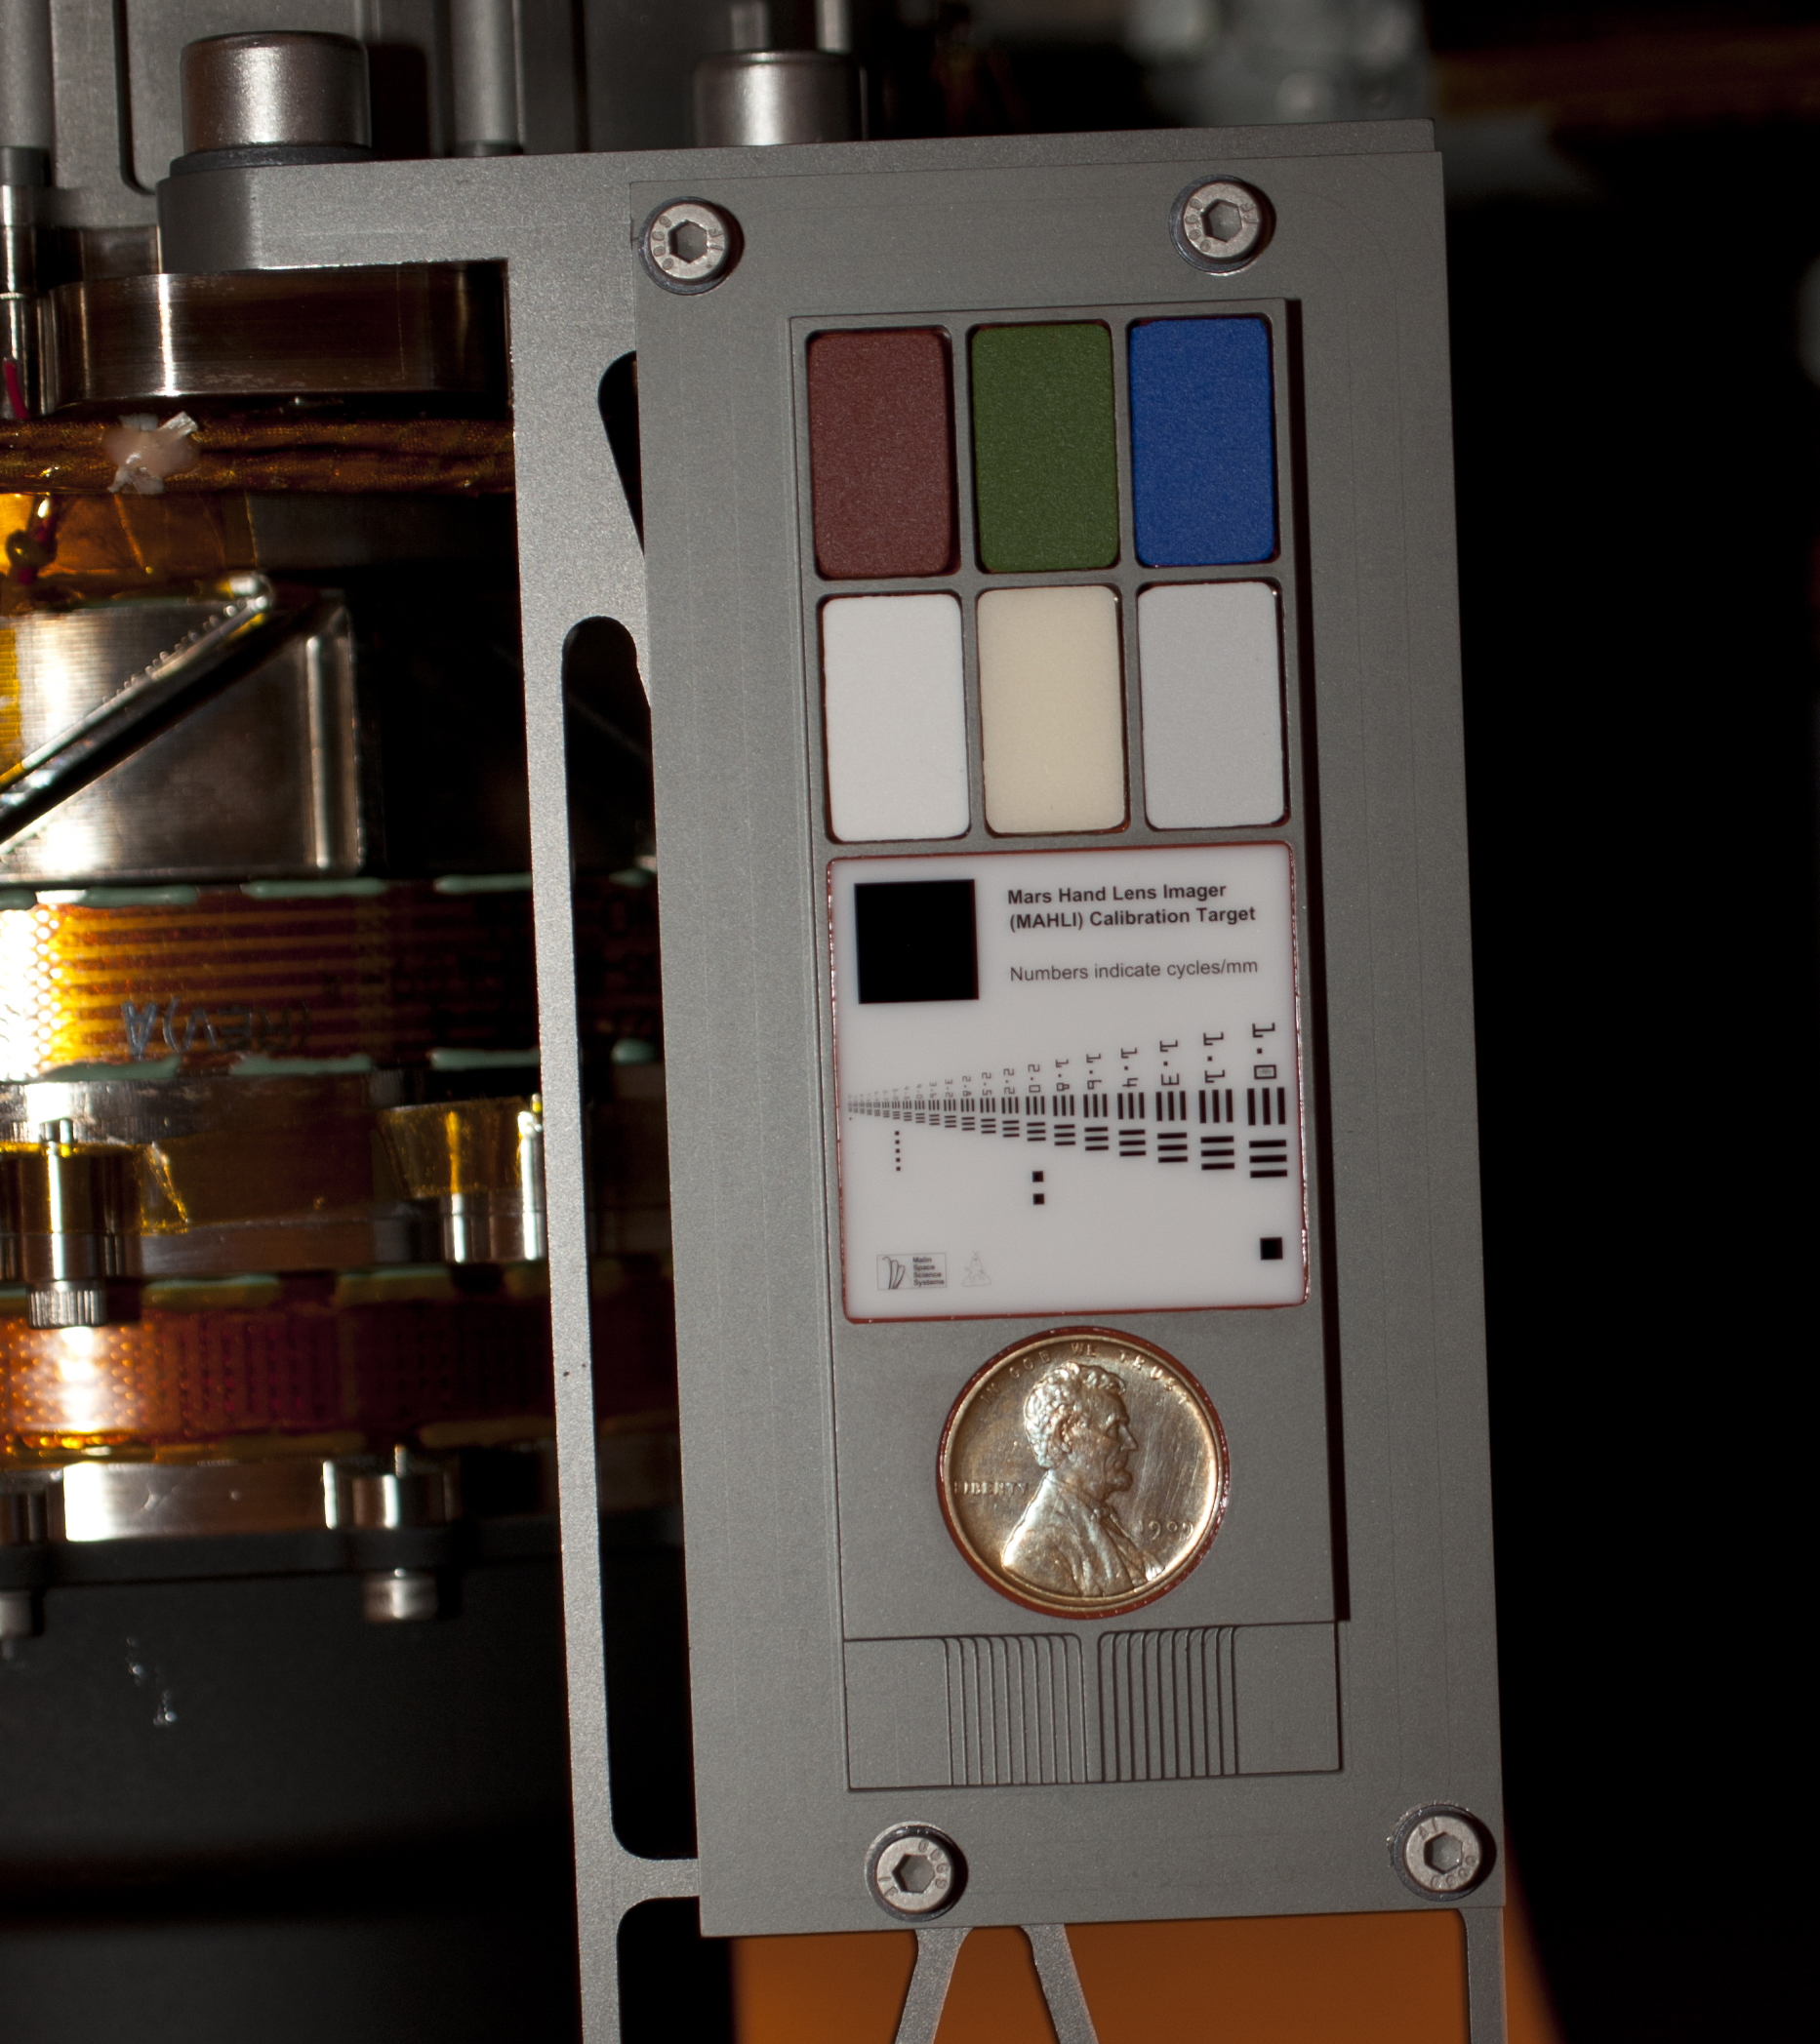
\includegraphics[width=7cm]{../images/curiosity_calibration_chart.jpg}
		\caption{Contact Instrument Calibration Targets on Mars Rover Curiosity \citep{curiosity_image_calibration}}
		\label{fig:curiosity_calibration_chart}
	\end{figure}\\\\
	The reference object must be located in the image using a technique such as BLOB analysis or Hough transforms. Once the object is found, its width or height in pixels in the image must be collected, as the real world size of this object is known then its width in pixels equates to this real world measurement in the image. For example, if 2mm wide object measures 424px across in an image then it can be concluded that 212px in the image are equal to 1mm. Any other objects that can be measured in pixels their real world measurement can be estimated if they are close to the same distance from the camera as the reference object.
	\\\\
	This process will be applied during this project in some manner, either using a reference object or measuring camera height, as knowing measurements is vital to suspension setup as previously stated. Implementation of equation \ref{equ:measureobj} in an application will be relatively simple though collection of the relevant data with as little user interaction as possible will be difficult.